\section{Inverted Index}
\label{sec:inverted-index}

An index can be seen as a matrix with the terms (e.g. unigram) for rows and the
collection's documents as columns. In this matrix, an element
equal to one if the term i occurs in document j, and zero if not. However such
a matrix contains practically only zeros, thus a lot of wasted space. Inverted
List is a basic IR structure that reduces such a matrix to only store ones'
values. All the inverted lists taken together form the inverted index.

From the collection a dictionary of the words appearing in is created. The
dictionary's terms have been first filtered, by removing the punctuation for
example. Given a term from the dictionary, a linked list is associated to it
and stores all documents records where the term occurs in. A document record
can be simply a serial number of the document (i.e., document identifier), but
additional information like the term frequency and the position can be given.
The term frequency corresponds to the number of occurrences of the term in a
document, and the position indicate the positions of the occurrences within
that document. The Figure~\ref{fig:inverted-list} depicts two inverted lists
storing documents identifiers as integers, term frequencies and positions.
These inverted lists are built using the terms ``killed'' and ``brutus'' from
documents in the Table~\ref{tab:indexing}. There
is a relation one-to-one between documents identifiers and term frequencies,
and a relation many-to-many with the positions. There are as much position
values as there are occurrences (i.e., term frequency) of the term in the
document. The documents identifiers are stored in increasing order in order
to process queries, as presented in Section~\ref{sec:query-model}.

\begin{figure}
\centering
\resizebox{0.8\linewidth}{!}{%
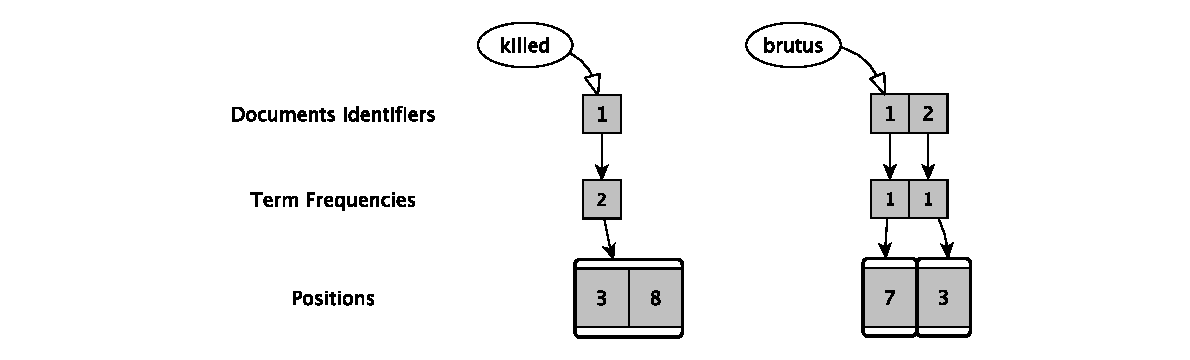
\includegraphics[scale=1]{pics/inverted-list}
}%
\caption{Inverted lists for the terms ``killed'' and ``brutus'' in documents
from the Table~\ref{tab:indexing}. Each inverted list stores the documents
identifiers, the term frequencies and the positions information.}
\label{fig:inverted-list}
\end{figure}

\subsection{Indexing}
\label{sec:IR-indexing}

In this section, traditional inverted index construction is presented, then the
block-based construction which makes possible to handle large collection.
Finally I discuss the importance of compression for large collection, and
present a commonly used  in Information Retrieval encoding technique.

An inverted index is the group of inverted lists built from a collection.
The basic steps to create an inverted index in the main memory from a collection
of documents are:
\begin{enumerate}
  \item make a first pass through the collection to gather term-document-i~dentifiers pairs
  \item sort the pairs with the term value as the key
  \item group together docIDs of a same term into an inverted list.
\end{enumerate}
These steps are reported in Table~\ref{tab:indexing} with two documents taken
from the ``Shakespeare's Collected Works'', storing only the document
identifier (docID) in the inverted lists and the document frequency (DF), i.e.
the number of documents the term appears in. Each words in the documents are
filtered by removing the punctuation and lowering the case. The set of terms
defines the dictionary of the inverted index. For each of the dictionary, an
inverted list is then created.

In order to build an inverted index once and for all, the in-memory
inverted index is written to the disk into what is called an \emph{inverted
file}. The Figure~\ref{fig:indexing} summarize the steps from the
collection to the creation of an inverted file. The inverted file contains all
the inverted lists, written one after the other. The dictionary is also stored
in that same file, where each term possess information about the inverted list
it points to: the inverted list's offset or the document frequency, i.e., the
number of documents the term appears in.

\begin{table}
\resizebox{\linewidth}{!}{%
\begin{tabular}{lrllrlllcl}
\toprule
\multicolumn{5}{l}{
{\bfseries Document 1:}
I was killed i' the Capitol; Brutus killed me.
}&
\multicolumn{5}{l}{
{\bfseries Document 2:}
The noble Brutus hath told you Caesar was ambitious.
}\\
\multicolumn{10}{c}{\phantom{a}}\\
{\bfseries term} & {\bfseries docID} & & {\bfseries term (sorted)} & {\bfseries
docID} & & {\bfseries term} & {\bfseries DF} & & {\bfseries Inverted List}\\
I & 1 & \multirow{18}{*}{$\Longrightarrow$} & ambitious & 2 &
\multirow{18}{*}{$\Longrightarrow$} & ambitious & 1 & $\mapsto$ & $1$ \\
was & 1 & & brutus & 1 & & brutus & 2 & $\mapsto$ & $1 \rightarrow 2$ \\
killed & 1 & & brutus & 2 & & capitol & 1 & $\mapsto$ & $1$ \\
i' & 1 & & capitol & 1 & & caesar & 1 & $\mapsto$ & $1$ \\
the & 1 & & caesar & 2 & & hath & 1 & $\mapsto$ & $1$ \\
capitol & 1 & & hath & 2 & & I & 1 & $\mapsto$ & 1 \\
brutus & 1 & & I & 1 & & i' & 1 & $\mapsto$ & $1$ \\
killed & 1 & & i' & 1 & & killed & 1 & $\mapsto$ & $1$ \\
me & 1 & & killed & 1 & & me & 1 & $\mapsto$ & $1$ \\
the & 2 & & killed & 1 & & noble & 1 & $\mapsto$ & $1$ \\
noble & 2 & & me & 1 & & the & 2 & $\mapsto$ & $1\rightarrow 2$ \\
brutus & 2 & & noble & 2 & & told & 1 & $\mapsto$ & $1$ \\
hath & 2 & & the & 1 & & you & 1 & $\mapsto$ & $1$ \\
told & 2 & & the & 2 & & was & 2 & $\mapsto$ & $1 \rightarrow 2$ \\
you & 2 & & told & 2 & & & & \\
caesar & 2 & &  you & 2 & & & & \\
was & 2 & & was & 1 & & & & \\
ambitious & 2 & & was & 2 & & & & \\
\bottomrule
\end{tabular}
}%
\caption{Inverted index creation from two documents taken in ``Shakespeare's
Collected Works''. Each word is filtered and associated to its document
identifier (docID). After sorting the pairs on the term, the inverted lists are
created for the set of terms. The inverted lists store only the docID of the
document the term appears in.}
\label{tab:indexing}
\end{table}

\begin{figure}
\centering
\resizebox{0.8\linewidth}{!}{%
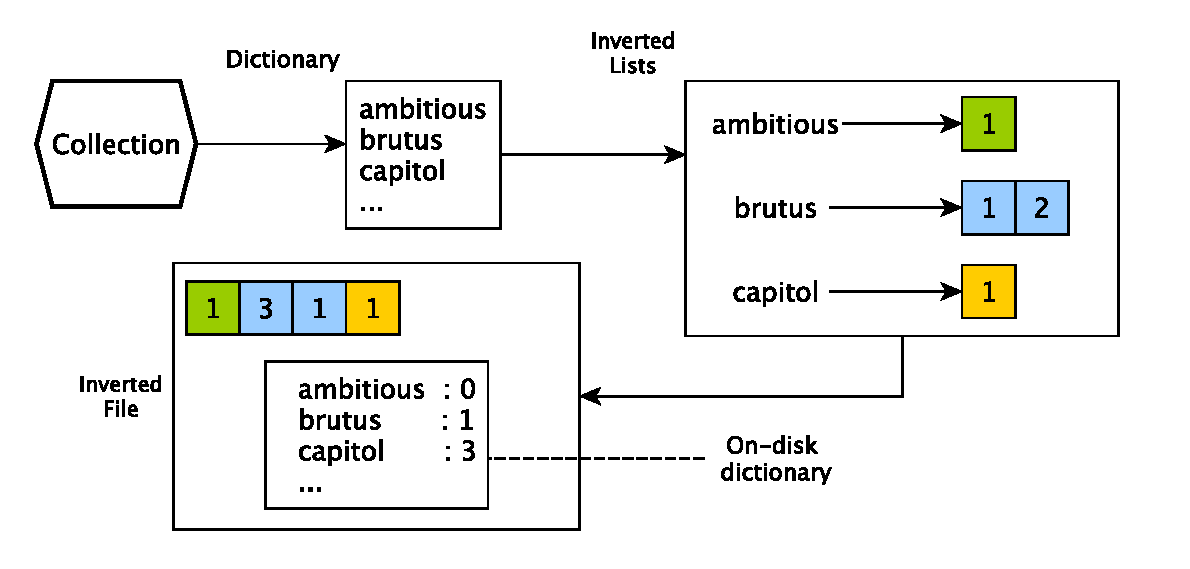
\includegraphics[scale=1]{pics/indexing}
}%
\caption{Indexing, from a collection of documents to the inverted file. The
in-memory inverted lists are written to disk one after the other. The
terms of the embedded dictionary possess offset to the associated inverted list
in the file.}
\label{fig:indexing}
\end{figure}

\subsubsection{Merge-Based Indexing}

The previous indexing technique works in-memory, and then cannot handle large
collection with large inverted lists. Merge-based indexing is a technique that
divides an inverted index construction into segments, which are then merged
together to form a complete inverted index. Thus an inverted list can span
over multiple segments. When the main memory is filled or that a threshold has
been reached, a segment is written to a secondary storage space (e.g. the disk)
into an inverted file. Each on-disk inverted file contains an inverted index
independent from the one in an other segment. When merging inverted files, it is
then necessary to update inverted lists of a same term but stored in different
segments. The Figure~\ref{fig:merged-indexing} depicts the merge process of
three inverted files into one. An inverted list spans over these files: the
documents identifiers values are then local to each file. Thus it is necessary
to update these identifiers numbers in order to keep an ordered inverted list
after merging.

Such an index construction requires two steps to finish. The first one consists
in building multiple segments and is called the \emph{commit} step. The second
one consists in the merging process of multiple files into one inverted file
and is called the \emph{optimization} step. These steps are believed to
be a common operation for incremental inverted index.

\begin{figure}
\centering
\resizebox{0.8\linewidth}{!}{%
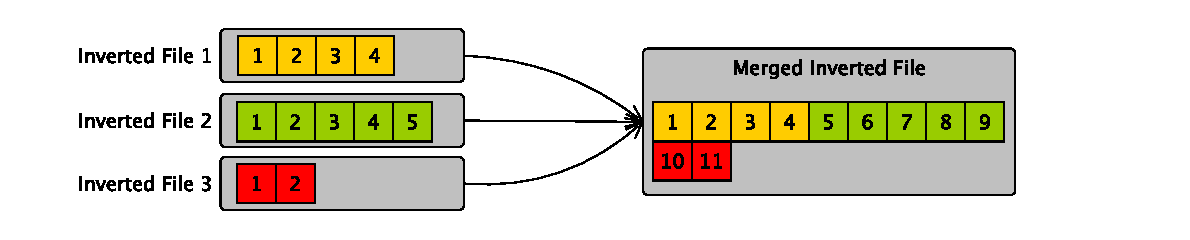
\includegraphics[scale=1]{pics/merged-indexing}
}%
\caption{Merge-based indexing of three inverted files. An inverted list, storing
documents identifiers, spans over these files. When merging these files into
one inverted file, the documents identifiers are updated to keep an ordered
list.}
\label{fig:merged-indexing}
\end{figure}

\subsubsection{Block-Based Inverted List}
\label{sec:compression:block}

For performance and compression efficiency, it is best to store separately each
data stream of an inverted list~\cite{anh:2006:siohttq}. In a non-interleaved
index organisation, the inverted index is composed of three inverted files,
one for each stream of values (i.e., documents identifiers, frequencies and
positions). Each inverted file stores contiguously one type of list, and three
pointers are associated to each term in the lexicon, one pointer to the
beginning of the list in each inverted file.

An inverted file is partitioned into blocks, each block containing a fixed
number of integers as shown in Figure~\ref{fig:index-structure}. Blocks are
the basic units for writing data to and fetching data from disk, but also the
basic data unit that will be compressed and decompressed. A block starts with
a block header. The block header is composed of the length of the block in
bytes and additional meta-data information that is specific to the compression
technique used. Long inverted lists are often stored across multiple blocks,
starting somewhere in one block and ending somewhere in another block, while
multiple small lists are often stored into a single block. For example, 16
inverted lists of 64 integers can be stored in a block of 1024 integers.

\begin{figure}
  \centering
	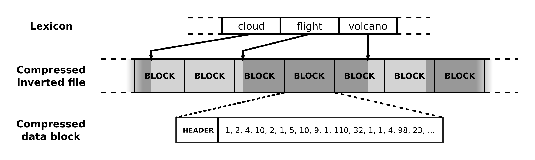
\includegraphics[scale=1.2]{pics/index-structure}
	\caption{Inverted index structure. Each lexicon entry (term) contains a
	pointer to the beginning of its inverted list in the compressed inverted
	file. An inverted file is divided into blocks of equal size, each block
	containing the same number of values.}
	\label{fig:index-structure}
\end{figure}

\subsubsection{Index Updates Strategies}

Updating the inverted index with new documents is done via two approaches: by
\emph{batches} or \emph{incrementally}.
The update strategy by batches stores
added documents into a buffer, and writes them to the index on-disk when some
threshold is reached. While this is adapted to static indexes, in other words
indexes that do not need to be updated right away. However in some cases such
as Internet news search engines, the user would expect the index to be updated
as soon new documents are detected. This use case is matched by incremental
updates strategy. With this strategy, the index is composed of the ones on
disk, but also with an index built in-memory. This second index holds the
updated documents temporarily that are bound to be written to the index on-disk
when a threshold is reached.
The question of deleted documents is handled thanks to a table that stores the
documents flagged in deleted state.

\subsection{Delta-Encoding}

Large collections result in large inverted files. As these files are stored on
disk, compressing their data is then crucial in order to save storage space.
\emph{Delta-encoding} is a basic encoding commonly used in Information
Retrieval which aims to decrease the size of inverted lists, thus reducing
inverted files disk space.

With an ordered and increasing list of integers, it is possible to considerably
reduce the size by storing not the actual integers values but the gaps. A gap
is the difference between two consecutive integers. As the list is increasing,
the difference between an integer at position $i$ and an integer at position
$i-1$ will always be positive. To decompress a value at position i from a
delta-compressed list, we just have to sum up every values up to i. The
Figure~\ref{fig:delta-encoding} depicts a delta-compressed list of integers. By
storing gaps values, we can reduce the size of the list from 88 to 38 bits.

Documents identifiers are stored in increasing order in each inverted list, and
can then be delta-encoded. Also the positions values are stored in increasing
order, but they are local to a document. Thus position values relative to a
same document are delta-encoded, and the encoding is re-initialized when
changing documents.

\begin{figure}
\centering
\resizebox{0.8\linewidth}{!}{%
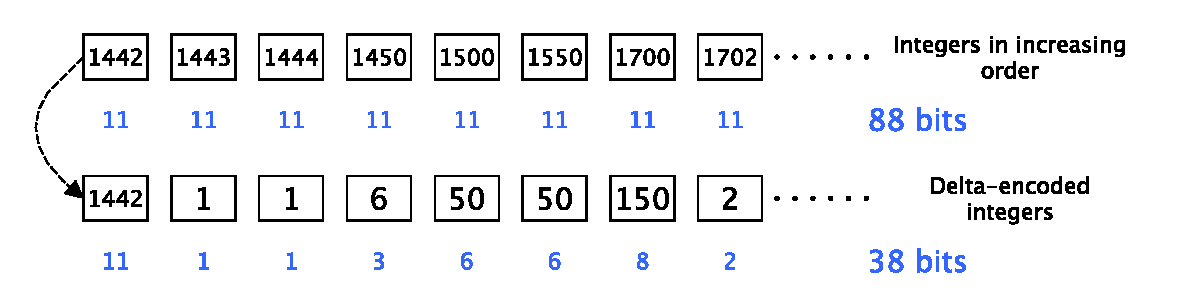
\includegraphics[scale=1]{pics/delta-encoding}
}%
\caption{Delta-encoding of an increasing ordered list of integers, showing the
size in bits of the two lists.}
\label{fig:delta-encoding}
\end{figure}

\section{Query Model}
\label{sec:query-model}

A query is an user request for information about the collection. Documents
matching that query are returned back to the user. In this section, I present
the query model used in Information Retrieval and explain how keyword and
Phrase queries are processed.

The model used to represent documents is the \emph{vector space model},
commonly called the ``bag of words'' model. In this model documents and
queries are seen as vectors, where a component represent a term in the
collection. Given a query and a set of document vectors, we compute the angle
between them. The smaller this angle is, the higher the document will be
ranked with regards to the query.

The query model is a Boolean model, where terms that are to appear in the
returned documents are combined together using Boolean operators. Boolean
operators include two binary operators, i.e., \emph{AND} and \emph{OR}, and one
unary operator \emph{NOT}. Their operands can be either a term or a Boolean
sequence of terms. With this model, documents in the indexed collection are
nothing more than a set of terms. Set theory operations are used to interpret
such queries. The Boolean operators are binary operations and their operands are
set of words. The And operator is interpreted as an \emph{Conjunction},
the OR operator as an \emph{Disjunction} and the NOT operator as the
\emph{Exclusion}. A simple Boolean query on the two documents from the
Table~\ref{tab:indexing}
\begin{center}
brutus \emph{AND} ambitious
\end{center}
searches for all documents containing the terms brutus and ambitious.

In this model, a document is seen as a \emph{bag of words}, where the exact
ordering of terms is ignored but the number of occurrences of each term (i.e.
term frequency) is material.

\subsection{Keyword Query Processing}

Keyword queries search for documents containing the terms in the Boolean
expression. Their processing follows the algorithm
\begin{enumerate}
  \item Retrieve inverted lists of all the query's terms.
  \item Apply set operations, i.e., union, intersection or set difference, on the
  inverted lists.
  \item Returns documents mapping to the documents identifiers in the inverted
  list, resulting of the set operations.
\end{enumerate}
The former query ``brutus AND ambitious'' returns the document identifier 1, as
the intersection of their inverted list give only this one identifier. The
Figure~\ref{fig:KWquery} depicts the processing of that query, showing in red
the documents identifiers occurring in both inverted lists.

\begin{figure}
\centering
\resizebox{0.35\linewidth}{!}{%
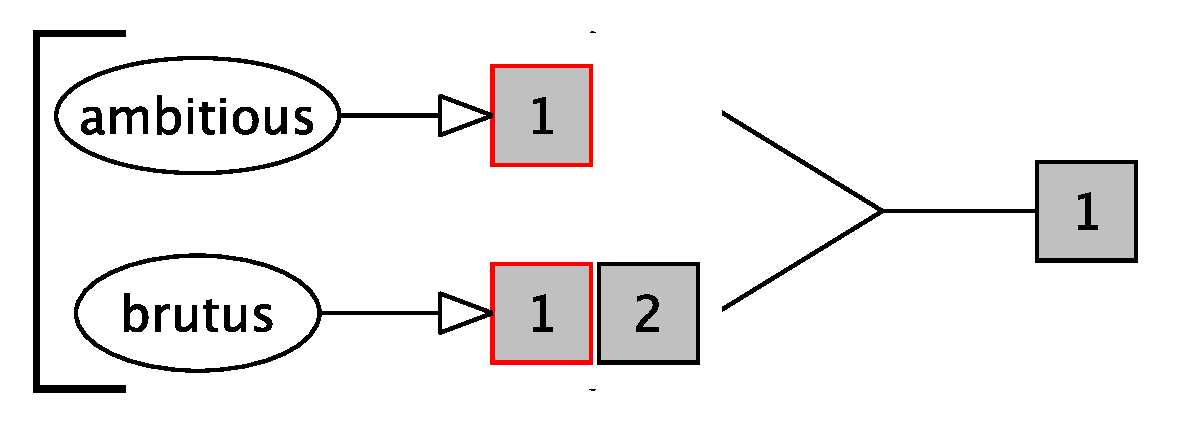
\includegraphics[scale=1]{pics/KWquery-processing}
}%
\caption{Processing of the keyword query ``brutus AND ambitious''. The only
document containing both terms is the document 1, from the
Table~\ref{tab:indexing}.}
\label{fig:KWquery}
\end{figure}

\subsection{Phrase Query Processing}

The position of terms in a document is very important, as it can change the
meaning of these terms in the document. For example the keyword query
``\emph{stanford AND university}'' may return a document containing the
sentence ``The inventor Stanford Ovshinsky never went to university''. However
the given query suggested to search information about a University in
Stanford. The returned document is then irrelevant to the query, to what really
is needed by the user. In order to perform more precise search, the position
information about the terms in documents is necessary. Indeed restricting the
search to documents having the keyword terms appear consecutively one after the
other will discard irrelevant documents. As four terms are between Stanford
and University in the former example, such a document will not be returned if
restricting to zero words in-between. The query that takes into account the
position of terms within documents are called \emph{Phrase queries}.

A \emph{n-gram} is a sub-sequence of n terms in the document. For instance, a
bi-gram (i.e., a sub-sequence of two terms) in document 1 in
Table~\ref{tab:indexing} can be ``I was'' or ``Brutus killed''. There exist
two ways to handle phrase queries. The first one relies on indexing n-gram
occurring in the collection. Indexing bi-gram would follow the same process as
in the Table~\ref{tab:indexing}, but with bi-gram instead of single terms.
However it restricts to bi-gram only, and to search for tri-gram (i.e., three
terms in the sub-sequence) it would mean to index also tri-gram. This is highly
inefficient as a huge storage space is then needed. The second way uses the
position information of terms within documents to process phrase queries. Thus
only uni-gram (i.e., one term in the sub-sequence) are indexed with the relative
position of each term. Also we can handle this way phrase queries with any
number of terms in the sub-sequence.

\subsubsection{Phrase queries processing algorithm}

The first step in processing phrase queries is the same as processing
keyword queries: after retrieving inverted lists of each term, we perform
operations on the inverted lists to get the list of documents identifiers
matching the terms in the query. The second step consists in filtering these
documents according to the position information. The algorithm to discard or
not a document works on the positions of keywords occurring in a same document,
and is as follows:
\begin{enumerate}
  \item[] Let R be the list of documents identifiers that results from the
  first step.
  \item For each document i in R.
  \item Retrieve the list $P_{T1,i}$ of positions for the term T1 in document i,
  and the list $P_{T2,i}$ of positions for the term T2 in document i.
  \item Compare position values $p_1 \in P_{T1,i}$ and $p_2 \in P_{T2,i}$
  \begin{enumerate}
    \item The absolute difference between $p_1$ and $p_2$ is \emph{greater than}
    1 $\Rightarrow$ within the list with the lower value, we advance until
    reading a position greater than the other value.
    \item The absolute difference between $p_1$ and $p_2$ is \emph{equal to} 1
    $\Rightarrow$ the current document is kept and we go to the next document
    in R.
  \end{enumerate}
\end{enumerate}
The Figure~\ref{fig:PQquery} depicts with dashed lines the comparisons performed
in the step 3 in the former algorithm. We first compare 1 and 8 and keep on
reading values in P1 until the value 20. Then the comparison between 20 and 8,
and so on. The algorithm stops at comparison 5, as the difference is equal to
1. The document is thus kept in the results of the phrase query. In the
Table~\ref{tab:indexing}, the phrase query ``brutus killed'' would match the
document 1, as the terms appear respectively in positions 7 and 8. We can note
that as the difference computed in steps 3 is absolute, the phrase query
``killed brutus'' also matches that document. This reflects the ``bag of
words'' query model in Information Retrieval.

\begin{figure}
\centering
\resizebox{0.9\linewidth}{!}{%
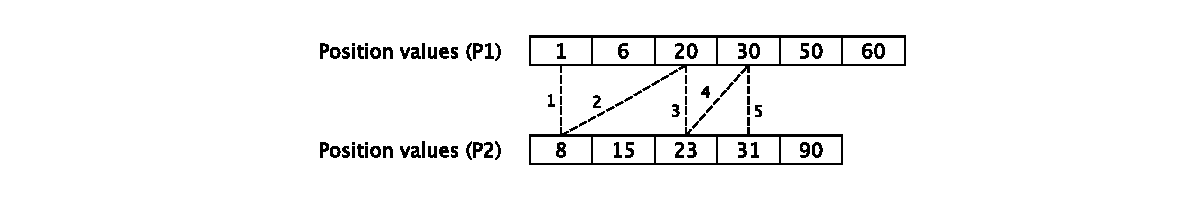
\includegraphics[scale=1]{pics/PQsearch}
}%
\caption{Documents filtering based on the position of terms. P1 and P2 are two
positions lists of two different terms occurring in the same document. Dashed
lines represent comparison between position values. The order in which these
comparisons are made is indicate by their label number.}
\label{fig:PQquery}
\end{figure}
